\section{A regular pentagon with a centrally symmetric partner}

The preceding result allows the two pentagons to deform independently.
We now keep one regular pentagon fixed and allow its partner to be any
centrally symmetric planar convex body, including a smooth body. The
capacity is then determined by a single convex-body inclusion. Its sharp
systolic ratio is strictly below one.

Use the preceding normal convention, writing
\[
 n_i=(\cos(2\pi i/5),\sin(2\pi i/5)),\qquad
 Q=\{p:n_i\cdot p\le h,\ 0\le i<5\},\qquad h=\cos(\pi/5).
\]
Thus $Q$ has circumradius one. For a convex body $A$ containing the origin
in its interior, write
$A^\circ=\{x:x\cdot y\le1\text{ for every }y\in A\}$.
Define
\[
 B=\tfrac12(Q-Q)^\circ
   =\operatorname{conv}\left\{\frac{\pm n_i}{2(1+h)}:0\le i<5\right\},
 \qquad
 W(K)=\max\{r\ge0:r(Q-Q)^\circ\subseteq K-K\}.
\]
The body $B$ is a regular decagon with its orientation fixed by $Q$.
The product below is Lagrangian, and $c$ denotes its
Ekeland--Hofer--Zehnder capacity.

\begin{theorem}
For every centrally symmetric planar convex body $K$ with nonempty interior,
\[
 c(K\times_L Q)=W(K),\qquad
 \frac{c(K\times_L Q)^2}{2\operatorname{area}(K)\operatorname{area}(Q)}
 \le \kappa_{\mathrm{sym}}:=\frac{10+6\sqrt5}{25}<1.
\]
Equality in the ratio holds exactly when $K$ is a translate of a positive
dilate of $B$.
\end{theorem}

The proof uses a translation-cover characterization of capacity.
For an oriented polygonal curve with edge vectors $v_j$, its $Q$-length is
$\sum_j s_Q(v_j)$, where $s_Q(v)=\max_{p\in Q}v\cdot p$.
This length can depend on orientation, since $Q$ is not symmetric.
Balitskiy--Mitrofanov--Polyanskii show that $c(K\times_L Q)\ge1$ exactly
when every closed curve of unit $Q$-length fits into a translate of $K$
\cite[Theorem 2.5]{BMP}.
For polygonal $Q$, it suffices to check the \emph{normal triangles}:
unit-length oriented triangles whose edges follow outward normal directions
of $Q$, including degenerate triangles when opposite normals exist
\cite[Definition 3.2 and Theorem 3.3]{BMP}. Our pentagon has no opposite
normals, so all its normal triangles are nondegenerate. There are ten translation
classes. Their underlying triangles have angles $\pi/5,\pi/5,3\pi/5$
and are rotations of one another through multiples of $\pi/5$
\cite[Section 6.1]{BMP}. For odd multiples, the traversal orientation
reverses so that the edges again follow outward normals.

\begin{proof}
We first compute $c(B\times_L Q)$. Put $\theta=\pi/5$ and
$R=1/[2(1+h)]$, the circumradius of $B$.
If a normal triangle has longest side $L$, its other sides both have length
$L/(2\cos\theta)$. Its oriented edges follow outward normals, so their
$Q$-lengths equal $h$ times their Euclidean lengths. Consequently
\[
 1=hL(1+1/\cos\theta)=L(1+h),\qquad L=2R.
\]
Translate the longest side's midpoint to the origin. Its endpoints are
antipodal vertices of $B$, and the third vertex has distance $R\tan\theta$
from the origin. This is smaller than the incircle radius $R\cos(\theta/2)$,
because
\[
 \tan^2(\pi/5)=5-2\sqrt5
       <\frac{5+\sqrt5}{8}=\cos^2(\pi/10).
\]
Each of the ten triangles therefore lies in $B$, giving $c(B\times_L Q)\ge1$.

\begin{figure}[H]
\centering
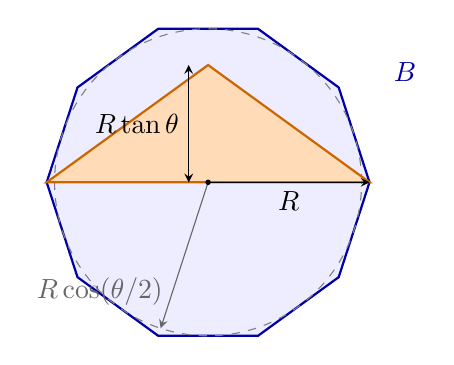
\begin{tikzpicture}[scale=2.05,>=stealth]
 \fill[blue!7] (0:1) \foreach \a in {36,72,...,324} {-- (\a:1)} -- cycle;
 \draw[blue!65!black,thick] (0:1) \foreach \a in {36,72,...,324} {-- (\a:1)} -- cycle;
 \draw[gray,dashed] (0,0) circle ({cos(18)});
 \filldraw[fill=orange!28,draw=orange!80!black,thick]
   (-1,0) -- (1,0) -- (0,{tan(36)}) -- cycle;
 \draw[->] (0,0) -- (1,0) node[midway,below] {$R$};
 \draw[<->] (-.12,0) -- (-.12,{tan(36)}) node[midway,left] {$R\tan\theta$};
 \draw[->,gray!80!black] (0,0) -- (252:{cos(18)})
    node[pos=.75,left] {$R\cos(\theta/2)$};
 \fill (0,0) circle (.017);
 \node[blue!65!black] at (1.22,.68) {$B$};
\end{tikzpicture}
\caption{A translated normal triangle in $B$. Its longest side joins
antipodal vertices; its third vertex lies inside the dashed incircle.
The same placement works after each rotation by $\pi/5$.}
\end{figure}

For any partner $K$, the curve-cover criterion gives the opposite bound
$c(K\times_L Q)\le W(K)$. Indeed, a segment traversed out and back with
displacement $v$ has length
$s_Q(v)+s_Q(-v)=s_{Q-Q}(v)$.
It fits into a translate of $K$ exactly when $v\in K-K$.
If capacity is at least $r>0$, rescale the first factor by $1/r$ and apply
the criterion to all unit-length segments. Convexity of $K-K$ then gives
$r(Q-Q)^\circ\subseteq K-K$.
Since $B-B=(Q-Q)^\circ$, this proves $c(B\times_L Q)=W(B)=1$.

Now translate a symmetric $K$ so that $K=-K$. Then $K-K=2K$, and the
definition of $W(K)$ gives $W(K)B\subseteq K$.
Monotonicity and homogeneity in one factor yield
$c(K\times_L Q)\ge W(K)c(B\times_L Q)=W(K)$,
proving the capacity formula.

The same containment gives
$\operatorname{area}(K)\ge W(K)^2\operatorname{area}(B)$.
Proper inclusion between full-dimensional convex bodies strictly increases
area, so equality holds exactly for translates of $W(K)B$.
Finally,
\[
 \operatorname{area}(B)=5R^2\sin(\pi/5),\qquad
 \operatorname{area}(Q)=\tfrac52\sin(2\pi/5),\qquad
 \frac1{2\operatorname{area}(B)\operatorname{area}(Q)}
    =\frac{10+6\sqrt5}{25}.
\]
This gives the sharp ratio and its equality class.
\end{proof}

The formula also identifies the bound $W$ for an asymmetric partner.
Its central symmetrization $S=(K-K)/2$ satisfies $S-S=K-K$, hence
\[
 W(K)=c(S\times_L Q),\qquad c(K\times_L Q)\le c(S\times_L Q).
\]
Thus the quotient $c(K\times_L Q)/W(K)$ records the fraction of the
symmetrized capacity retained by $K$.
In particular, a counterexample with this fixed pentagon factor must use
an asymmetric partner. The argument explains this restriction by calibrating
one reference cover and transferring its capacity through containment.
